\PassOptionsToPackage{table}{xcolor} % Somente para o uso do Victor, Comente esta linha e descomente a linha do Base.tex \usepackage[table]{xcolor}
\documentclass{beamer}

%Arquivo com os principais pacotes usados e suas descrições.

%%%%%%%%%%%%%%%%%%%%%%%%%%%%%%%%%%%%%%%%%
% 			Idiomas e Acentos			%
%%%%%%%%%%%%%%%%%%%%%%%%%%%%%%%%%%%%%%%%%
\usepackage[brazil]{babel} % Habilita o uso do idioma português do brasil (PT-BR).
\usepackage[T1]{fontenc} 
%\usepackage{fontspec} % Habilita maior variedade de acentos. Pode ser necessario adicionar outros pacotes.
\usepackage{lmodern} % Habilita o uso da font Latin Modern.


%%%%%%%%%%%%%%%%%%%%%%%%%%%%%%%%%%%%%%%%%
% 				TABELAS					%
%%%%%%%%%%%%%%%%%%%%%%%%%%%%%%%%%%%%%%%%%
\usepackage{tabulary} % Cria tabelas mais facilmente.
\usepackage{booktabs} % Melhora o visual das tabelas.
\usepackage{table}{xcolor} % Pacote de cor pra as tabelas.
\usepackage{caption} % Melhora as legendas de imagens, tabela etc.

%%%%%%%%%%%%%%%%%%%%%%%%%%%%%%%%%%%%%%%%%
% 				IMAGENS					%
%%%%%%%%%%%%%%%%%%%%%%%%%%%%%%%%%%%%%%%%%
%\usepackage{graphicx} % Facilita a inserção de imagens.


%%%%%%%%%%%%%%%%%%%%%%%%%%%%%%%%%%%%%%%%%
% 			CÓDIGO FONTE				%
%%%%%%%%%%%%%%%%%%%%%%%%%%%%%%%%%%%%%%%%%
%Documentação de código fonte.
\usepackage{listings}


%%%%%%%%%%%%%%%%%%%%%%%%%%%%%%%%%%%%%%%%%
% 	Símbolos e Caracteres Matemáticos	%
%%%%%%%%%%%%%%%%%%%%%%%%%%%%%%%%%%%%%%%%%
\usepackage{amsmath}
\usepackage{amssymb}
\usepackage{amsfonts}
%\usepackage{mathspec} %Habilita o uso das fontes e dos caracteres matematicos.


%%%%%%%%%%%%%%%%%%%%%%%%%%%%%%%%%%%%%%%%%
%				ABNT					%
%%%%%%%%%%%%%%%%%%%%%%%%%%%%%%%%%%%%%%%%%
%\usepackage[alf]{abntcite} % Ordena as referencias em ordem alfabética.
\usepackage{url} %Facilita o uso de url. Pode-se usar o comando \url{...}.


%%%%%%%%%%%%%%%%%%%%%%%%%%%%%%%%%%%%%%%%%
% 			Configurações				%
%%%%%%%%%%%%%%%%%%%%%%%%%%%%%%%%%%%%%%%%%
\captionsetup{justification=centering,labelfont=bf} %Formata a legenda das figuras.
%\graphicspath{{../imgs/}} %Define o diretorio padrão para buscar as imagens da apresentação.  
%\setromanfont[Ligatures=TeX]{Crimson}
%\defaultfontfeatures{Scale=MatchLowercase, Mapping=tex-tex}

%%%%%%%%%%%%%%%%%%%%%%%%%%%%%%%%%%%%%%%%%
%				BEAMER					%
%%%%%%%%%%%%%%%%%%%%%%%%%%%%%%%%%%%%%%%%%
%Define algumas configurações que serão validas para todo o documento.  
\setbeamertemplate{section in toc}[sections numbered]
\setbeamertemplate{subsection in toc}[subsections numbered]
\setbeamertemplate{background canvas}[vertical shading][bottom=blue!3,top=blue!7]
\setbeamertemplate{caption}[numbered]


\author{ Denis F. de Carvalho \\
	 Guilherme A. de Macedo \\
	 Matheus L. D. da Silva \\
	 Victor H. Carlquist da Silva
}

\title{ Seis Sigma }
\date{\today}

\begin{document}

	\frame{
		\titlepage
	}

	\frame{
		\frametitle{Introdução}
		
		Seis Sigma é um programa de melhoria de processo baseado em uma metodologia de solução de problemas.
		\begin{itemize}
			\item Definição;
			\item Medição;
			\item Análise;
			\item Melhoria;
			\item Controle.
		\end{itemize}
		
	}
	\frame{
		\frametitle{História}
		\begin {itemize}
			\item Datado de 1809 - Carl Gauss;
			\item \textit{Theoria Motus Corporum Arithmeticae} - Curva do sino;
			\item Motorola em crise - 1986;
			\item Motorola ganha prêmio Malcolm Baldridge National Quality Award - 1988;
		\end{itemize}
	}
	\frame{
		\frametitle{Níveis de Sigma}
		\begin{table}
			%\rowcolors{2}{gray!10}{white}
				\begin{tabular}{rcr}
					\toprule
					Sigma & Problemas por Milhão (PPM) & Porcentagem (\%) \\
					\midrule
					 1 & 697700	& 30,23 	\\
					 2 & 308700 & 69,13 	\\
					 3 & 66810 	& 93,32 	\\
					 4 & 6210 	& 99,379 	\\
					 5 & 233 	& 99,9767 	\\
					 6 & 3,4 	& 99,99966 	\\
					\bottomrule		
				\end{tabular}
	
				\label{tab_niveisSigma}
				\caption{Níveis de Sigma.}
				
			\end{table}
	}
	\frame{
	    \frametitle{Curva Normal}
	    \begin{figure}
	        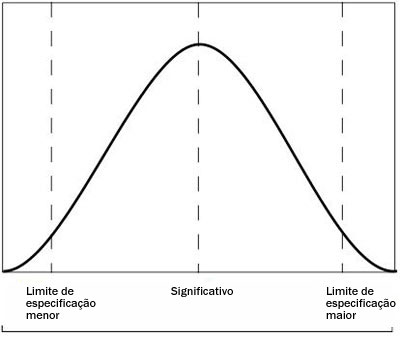
\includegraphics[width = 7cm,keepaspectratio]{../pesquisa/img/curva.jpg}
	        \caption{Curva Normal.}
	    \end{figure}
	
	}
	\frame{
		\frametitle{Metodologia}
		O Seis Sigma é composto, basicamente, por duas metodologias:
		\begin{itemize}
		    \item DMAIC;
		    \item DMADV.
		\end{itemize}
	}
	\frame{
		\frametitle{DMAIC}
        DMAIC
        \begin{enumerate}
            \item Definir (\textit{Define});
            \item Medir (\textit{Measure});
            \item Analisar (\textit{Analyse});
            \item Melhorar (\textit{Improve});
            \item Controlar (\textit{Control});
        \end{enumerate}
	}
	\frame{
		\frametitle{DMADV}
		DMADV
        \begin{enumerate}
            \item Definir (\textit{Define});
            \item Medir (\textit{Measure});
            \item Analisar (\textit{Analyse});
            \item Projetar (\textit{Design});
            \item Verificar (\textit{Verify});
        \end{enumerate}
	}
	\frame{
		\frametitle{DMAIC x DMADV}
		\begin{itemize}
		    \item Principais Semalhanças;
	        \item Principais Diferenças.
	    \end{itemize}
	}
	\frame{
		\frametitle{Conclusão}
	    ??????????????????
	}

\end{document}
		
